%!TEX root = ./main.tex
\chapter{Simulações 2D}
\label{simulacoes}

Para dar continuidade às simulações 2D introduzidas no relatório anterior, centenas de simulações foram realizadas para estudar subdução e três simulações chaves serão apresentadas neste capítulo. O objetivo é realizar uma investigação paramétrica para quantificar os fatores que contribuem para a dinâmica da subducção, entender como o código \textit{Mandyoc} \citep{sacek2022mandyoc} consegue reproduzir os cenários, comparar os resultados aqueles do trabalho de \citet{strak2021thermo}, e estudar um cenário de subdução análogo aquele observado na América do Sul, onde a placa de Nazca subduz sob a placa da América do Sul. Dito isso, vale ressaltar que as simulações que serão apresentadas têm caráter de teste.

% O primeiro desses parâmetros a serem investigados é o papel da reologia do manto superior no processo de subducção, que está diretamente associado à velocidade de subducção e sua variação no tempo \citep{strak2021thermo}.

% O segundo parâmetro é a resistência (ou força) da interface de subducção, que controla o ângulo de subducção, a velocidade de subducção e a taxa de \textit{rollback}. Além de outros fatores, a resistência da interface de subducção depende da quantidade de sedimento subduzido \citep{erdosetal2021role}.

% E o terceiro e último parâmetro é a fragilização térmica da litosfera em subducção. Ainda mal compreendido, esse parâmetro deve estar associado ao acoplamento da litosfera descendente na descontinuidade de 660 km. A princípio, a fragilização térmica deve ser considerada apenas nos estágios mais avançados das simulações.

% Para estudar esses parâmetros, pretendo criar um modelo numérico de subducção cuja dinâmica seja governada pela flutuabilidade da litosfera descendente (\textit{buoyancy-driven}) usando o código \textit{Mandyoc}. Utilizando uma geometria 2D simplificada, as simulações devem permitir fazer mudanças nas espessuras crustais e litosféricas com facilidade, contribuindo para simular o trecho central da zona de subducção da América do Sul. Embora o estudo 3D seja ideal, a abordagem 2D é apropriada para regiões centrais em zona de subducção relativamente extensas \citep{strak2021thermo}. %Esse tipo de modelo é tipicamente largo e profundo, com as litosferas envolvidas livres na superfície do modelo, e por isso os resultados são apresentados como recortes do modelo maior. 

% A tabela \ref{table:parametrosSimulacao} mostra os parâmetros físicos utilizados para a criação das configurações inciais e a figura \ref{fig:geometria} representa a geometria da simulação. 

% \begin{figure}[htb]
%   \begin{center}
%     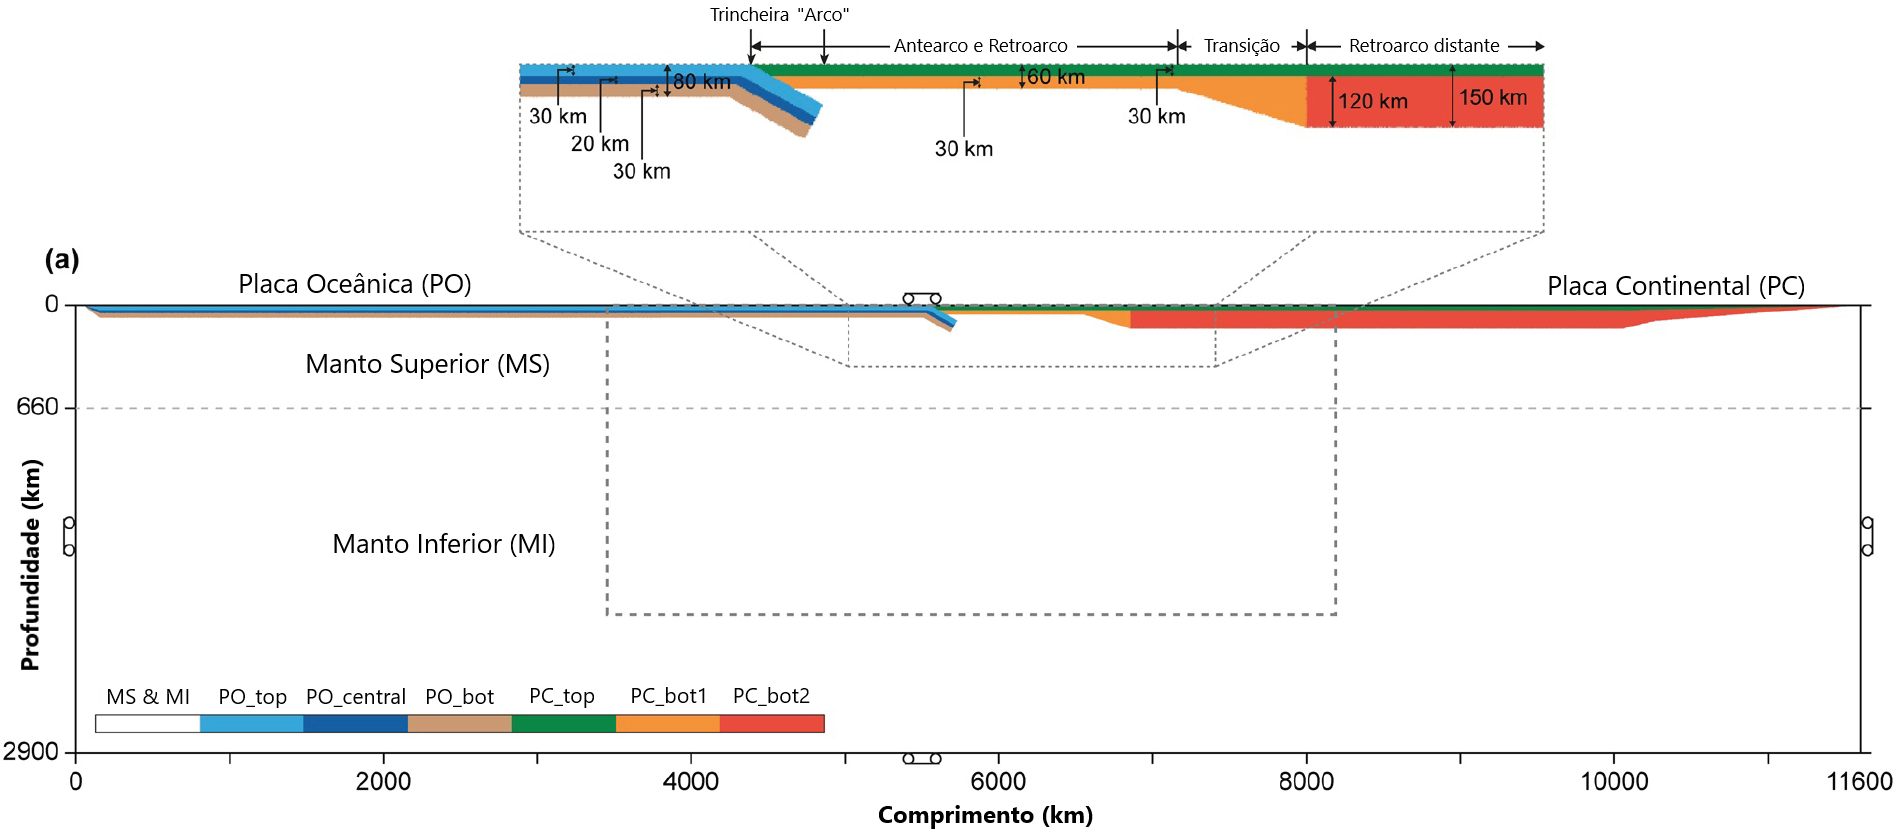
\includegraphics[width=1.0 \columnwidth]{fig/geometria.png}
%   	\caption{\label{fig:geometria}Geometria usada para as simulações indicando as diferentes unidades composicionais, adaptado de \citet{strak2021thermo}.}
%   \end{center}
% \end{figure}

% \begin{center}
    \setcaptionmargin{1cm}
    \scriptsize
    \begin{longtable}{lccccccc}
        \caption[Parâmetros de simulação \citep{strak2021thermo}.]{Parâmetros de simulação \citep{strak2021thermo}. MS, PO e PC são acrônimos para manto superior, placa oceânica e placa continental, respectivamente.}\\
        \hline \hline \\[-2ex]
        \multicolumn{1}{c}{Parâmetro} &
        \multicolumn{1}{c}{Símbolo} &
        \multicolumn{1}{c}{Valor} &

        \\[0.5ex] \hline
        \\[-1.8ex]
        
        \endfirsthead
        
        \multicolumn{4}{c}{\footnotesize{{\slshape{{\tablename} \thetable{}}} - Continuação}}\\[0.5ex]
        
        \hline \hline\\[-2ex]
        
        \multicolumn{1}{c}{Parâmetro} &
        \multicolumn{1}{c}{Símbolo} &
        \multicolumn{1}{c}{Valor} &
        
        \\[0.5ex] \hline
        \\[-1.8ex]
        
        \endhead
        
        \multicolumn{5}{l}{{\footnotesize{Continua na próxima página\ldots}}}\\
        \endfoot
        \hline
        
        \endlastfoot

        Largura do modelo & $l$ & $6000$ km \\
        Altura do modelo & $h$ & $1040$ km \\
        Ângulo de subdução & $h$ & $29$º \\

        Espessura crustal (PO) & $t_{PO,C}$ & $30$ km \\
        Espessura litosférica (PO) & $t_{PO,L}$ & $20$ km \\
        Extensão dorsal (PO) & $l_{PO,D}$ & $20$ km \\
        Extensão normal (PO) & $l_{PO,N}$ & $20$ km \\
        Extensão da subdução & $l_{PO,S}$ & $200$ km \\
    
        Espessura crustal (AC) & $t_{AC,C}$ & $30$ km \\
        Espessura litosférica (AC) & $t_{AC,L}$ & $30$ km \\
        Extensão arco (AC) & $l_{AC}$ & $30$ km \\

        Espessura crustal (C) & $t_{C,C}$ & $30$ km \\
        Espessura litosférica (C) & $t_{C,L}$ & $30$ km \\
        Extensão flanco esquerdo (C) & $l_{C,FE}$ & $30$ km \\
        Extensão centro cratônico (C) & $l_{C,CC}$ & $30$ km \\
        Extensão flanco direito (C) & $l_{C,FD}$ & $30$ km \\
        
        Densidade de referência & $\rho_r$ & $3230$ kg cm$^{-3}$ \\
        Densidade do ar & $\rho_r$ & $3230$ kg cm$^{-3}$ \\
        Densidade da crosta oceânica & $\rho_r$ & $3230$ kg cm$^{-3}$ \\
        Densidade do manto litosférico oceânico & $\rho_r$ & $3230$ kg cm$^{-3}$ \\
        Densidade da crosta continental & $\rho_r$ & $3230$ kg cm$^{-3}$ \\
        Densidade do manto litosférico continental & $\rho_r$ & $3230$ kg cm$^{-3}$ \\
        Densidade do manto astenosférico & $\rho_r$ & $3230$ kg cm$^{-3}$ \\
        Densidade do manto inferior & $\rho_r$ & $3230$ kg cm$^{-3}$ \\

        Aceleração da gravidade & $g$ & $10$ m s$^{-2}$ \\
        Coeficiente de expansão térmica & $\alpha$ & $1\times10^{-5}$ K$^{-1}$ \\
        Coeficiente de difusão térmica & $\kappa$ & $1\times10^{-5}$ m$^2$ s$^{-1}$ \\

        Viscosidade de referência (MS) & $\eta_{ref}$ & $3.5 \times 10^{20}$ Pa s \\
        Viscosidade mínima (MS) & $\eta_{MS,min}$ & $3.5 \times 10^{19}$ Pa s \\
        Viscosidade máxima (MS) & $\eta_{MS,max}$ & $3.5 \times 10^{20}$ Pa s \\
        Viscosidade do manto inferior & $\eta_{MI}$ & $3.5 \times 10^{22}$ Pa s \\
        Viscosidade da camada superior (PO) & $\eta_{PO,top}$ & $3.5 \times 10^{23}$ Pa s \\
        Viscosidade da crosta (PC) & $\eta_{PC,crosta}$ & $3.5 \times 10^{23}$ Pa s \\
        Viscosidade da camada central (PO) & $\eta_{PO,central}$ & $3.5 \times 10^{23}$ Pa s \\
        Viscosidade da camada inferior (PO) & $\eta_{PO,bot}$ & $1.75 \times 10^{22}$ Pa s \\
        Viscosidade da camada eclogitizada (PO) & $\eta_{PO,eclo}$ & $1.75 \times 10^{22}$ Pa s \\
        Viscosidade do manto litosférico no antearco e retroarco  (PC) & $\eta_{PC,arcos}$ & $1.4 \times 10^{23}$ Pa s \\
        Viscosidade do manto litosférico no retroarco distante (PC) & $\eta_{ps,dist}$ & $7 \times 10^{23}$ Pa s \\
        Tensão de ruptura da camada superior (PO) & $\sigma_{y}$ & $21$ MPa \\
        Fator pré-exponencial & $A$ & $3\times 10^{6}$ Pa$^n$ s \\
        Energia de ativação do manto superior & $E$ & $530\times 10^3$ J mol$^{-1}$ \\
        Constante dos gases & $R$ & $8.3145$ J mol$^{-1}$ K$^{-1}$ \\

        \label{table:parametrosSimulacao}
    \end{longtable}
\end{center} 

Para realizar as simulações, escrevi um \textit{Notebook} utilizando \textit{JupyterLab} (\url{https://jupyter.org}) para construir um modelo inicial que contém diferentes unidades litológicas, cada uma com um conjunto de propriedades físicas. Como ponto de partida, o \textit{script} constrói limites litológicos, calcula um campo de temperatura inicial e constrói um arquivo de parâmetros \textit{param.txt} para ser utilizados pelo código \textit{Mandyoc}. As simulações foram feitas no Cluster Aguia4 (\url{https://hpc.usp.br}).

O \textit{Notebook} está disponível na minha página do \textit{GitHub} no \textit{link} \url{https://github.com/jamisonassuncao/mandyoc-scripts}. A página também contém outros dois \textit{scripts} que escrevi, um para visualização dos arquivos do \textit{Mandyoc} e outro, em desenvolvimento, para utilizar os modelos LITHO1.0 \citep{pasyanos2014litho1} e Slab2 \citep{hayes2018slab2} para espessuras crustal e litosférica de toda América do Sul.

% O \textit{script subduction-initial.ipynb} do repositório cria unidades litológicas com diferentes espessuras e propriedades com o objetivo de produzir um cenário inicial para subdução. 

\section{Geometria}

A geometria das unidades litológicas é simplificada e contém uma litosfera oceânica à esquerda de uma litosfera continental, cada uma com duas camadas, como esquematiza a figura \ref{fig:geometria-inicial}. A camada superior de cada uma representa a crosta e a camada inferior representa o manto litosférico. Acima de ambas, uma camada de ar de $40$ km também foi definida. Note que existem duas camadas de astenosfera na figura \ref{fig:geometria-inicial}; isso é necessário porque o \textit{Mandyoc} necessita que todas as camadas sejam desenhadas da esquerda para a direita, exigindo que algumas camadas tenham que segmentadas.

\begin{figure}
    \centering
    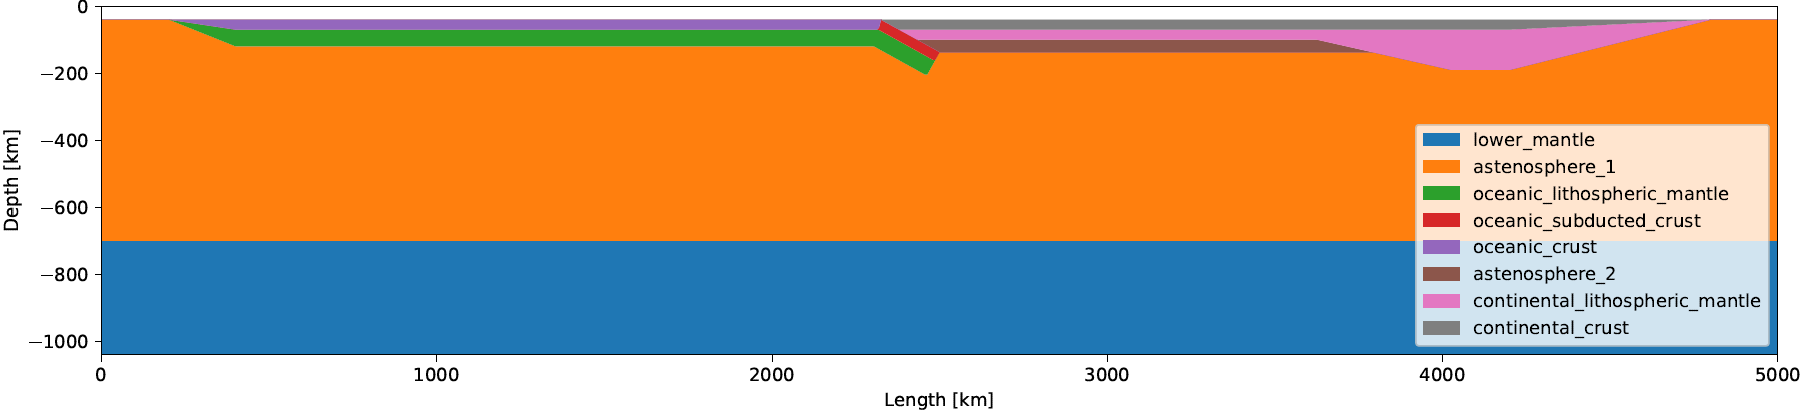
\includegraphics[width=1.0 \textwidth]{fig/geometria-inicial.png}
    \caption{Exemplo de geometria inicial das diferentes unidades litológicas utilizadas para simulação. A camada branca representa o ar.}
    \label{fig:geometria-inicial}
\end{figure}

Na placa oceânica há três trechos importantes, um trecho de espessamento litosférico, um trecho de espessura constante e, por último, um trecho em subdução sob a litosfera continental. A placa oceânica foi posicionada a $100$ km de distância da borda do modelo para evitar ancoramento da litosfera e seu trecho de espessamento representa a geometria simplificada de uma dorsal, havendo \textit{ridge-push} da esquerda para a direita no modelo.

Na placa continental há duas regiões a serem destacadas: uma região de arco continental e uma região cratônica. Na região de arco continental a litosfera apresenta uma espessura constante e é relativamente mais fina do que a região cratônica. Na região cratônica, por sua vez, há dois trechos de espessamento, uma entre o arco continental e o cráton, e outro entre o cráton e a superfície. 

A abordagem utilizada para a execução da simulação considerou que a placa oceânica, que avança de oeste para leste, mergulha para o interior do planeta devido ao \textit{slab-pull}. Para isso, todas as velocidades evoluem dinamicamente durante a simulação, \textit{free slab approach} \citep{assuncao2019}.

\section{Estrutura térmica}

A configuração térmica inicial é bastante simples ao passo que a temperatura é $0^{\circ}$C para toda a camada de ar e varia linearmente de $0$ºC na superfície até $1300$ºC no limite litosfera-astenosfera (\textit{Lithosphere-Astenosphere Boundary}, LAB). Para profundidades maiores do que o LAB, a temperatura considerada é a temperatura adiabática tal como na equação \ref{eq:adiabatic-temp} \citep{turcotte2002geodynamics}.

\begin{equation}{}\label{eq:adiabatic-temp}
  T = T_0 \exp{\frac{\alpha g z}{C_p}}
\end{equation}

% A escolha de tal configuração permite que a subducção ocorra por flutuabilidade térmica e seja independente dos efeitos das variações verticais de densidade e temperatura \citep{strak2021thermo}.

\section{Reologia}

As simulações numéricas propostas são simulações de sistemas isolados, onde todas as forças, propulsoras e resistivas, estão contidas no domínio do modelo. Esse tipo de abordagem garante que a convecção no modelo seja resultado dos contrastes de densidade causados pelo campo de temperatura.

Para um fluxo de arrasto característico do manto terrestre, a componente dúctil da viscosidade pode ser calculada utilizando a lei de Arrhenius ao desconsiderar o efeito da pressão tal como na equação \ref{power-law} da seção \ref{sec:reologia} \citep{vankeken2008community}. Dessa forma, a lei de potência pode ser representada pela equação \ref{power-law-2} a seguir.
\begin{equation}{\label{power-law-2}}
	\eta = \frac{1}{2} A^{\frac{-1}{n}} \dot{\varepsilon_{II}}^{\frac{1-n}{n}} \exp{\frac{Q}{nRT}} 
\end{equation}
%\noindent onde $\eta$ é a viscosidade efetiva, $A$ é o fator pré-exponencial, $n$ é o expoente da lei de potência, $Q$ é a energia de ativação, $R$ é a constante universal dos gases e $\dot{\varepsilon_{II}}$ é o segundo invariante do tensor taxa de deformação deviatória. 
% Vale ressaltar que para $n=1$, a equação \ref{power-law-2} representa a viscosidade efetiva para um fluido Newtoniano e, neste estudo, o fluido não-Newtoniano possui $n=3.5$.

% Já a componente rúptil proposta no trabalho de \citet{strak2021thermo} vale $\tau_{yield}=21$ MPa e segue o critério de von Mises tal como na equação \ref{viscosidade-efetiva} da seção \ref{sec:reologia}.

[FALAR DA FRAGILIZAÇÃO AQUI]

\section{Discussão}

Para prosseguir com a discussão de algumas simulações, um modelo de referência (MR) será discutido e seus parâmetros de simulação são apresentados na tabela \ref{table:referencia}. Este modelo é ponto de partida para entender os parâmetros simulados e também as mudanças na abordagem de simulações futuras. Vale ressaltar que as simulações apresentadas neste relatório são parte de um grupo de centenas de simulações e a sequência apresentada aqui é apenas de apresentação.

\begin{center}
    \setcaptionmargin{1cm}
    \scriptsize
    \begin{longtable}{lccccccc}
        \caption[Parâmetros de simulação \citep{strak2021thermo}.]{Parâmetros de simulação \citep{strak2021thermo}. MS, PO e PC são acrônimos para manto superior, placa oceânica e placa continental, respectivamente.}\\
        \hline \hline \\[-2ex]
        \multicolumn{1}{c}{Parâmetro} &
        \multicolumn{1}{c}{Símbolo} &
        \multicolumn{1}{c}{Valor} &

        \\[0.5ex] \hline
        \\[-1.8ex]
        
        \endfirsthead
        
        \multicolumn{4}{c}{\footnotesize{{\slshape{{\tablename} \thetable{}}} - Continuação}}\\[0.5ex]
        
        \hline \hline\\[-2ex]
        
        \multicolumn{1}{c}{Parâmetro} &
        \multicolumn{1}{c}{Símbolo} &
        \multicolumn{1}{c}{Valor} &
        
        \\[0.5ex] \hline
        \\[-1.8ex]
        
        \endhead
        
        \multicolumn{5}{l}{{\footnotesize{Continua na próxima página\ldots}}}\\
        \endfoot
        \hline
        
        \endlastfoot

        Largura do modelo & $l$ & $6000$ km \\
        Altura do modelo & $h$ & $1040$ km \\
        Ângulo de subdução & $h$ & $29$º \\

        Espessura crustal (PO) & $t_{PO,C}$ & $30$ km \\
        Espessura litosférica (PO) & $t_{PO,L}$ & $20$ km \\
        Extensão dorsal (PO) & $l_{PO,D}$ & $20$ km \\
        Extensão normal (PO) & $l_{PO,N}$ & $20$ km \\
        Extensão da subdução & $l_{PO,S}$ & $200$ km \\
    
        Espessura crustal (AC) & $t_{AC,C}$ & $30$ km \\
        Espessura litosférica (AC) & $t_{AC,L}$ & $30$ km \\
        Extensão arco (AC) & $l_{AC}$ & $30$ km \\

        Espessura crustal (C) & $t_{C,C}$ & $30$ km \\
        Espessura litosférica (C) & $t_{C,L}$ & $30$ km \\
        Extensão flanco esquerdo (C) & $l_{C,FE}$ & $30$ km \\
        Extensão centro cratônico (C) & $l_{C,CC}$ & $30$ km \\
        Extensão flanco direito (C) & $l_{C,FD}$ & $30$ km \\
        
        Densidade de referência & $\rho_r$ & $3230$ kg cm$^{-3}$ \\
        Densidade do ar & $\rho_r$ & $3230$ kg cm$^{-3}$ \\
        Densidade da crosta oceânica & $\rho_r$ & $3230$ kg cm$^{-3}$ \\
        Densidade do manto litosférico oceânico & $\rho_r$ & $3230$ kg cm$^{-3}$ \\
        Densidade da crosta continental & $\rho_r$ & $3230$ kg cm$^{-3}$ \\
        Densidade do manto litosférico continental & $\rho_r$ & $3230$ kg cm$^{-3}$ \\
        Densidade do manto astenosférico & $\rho_r$ & $3230$ kg cm$^{-3}$ \\
        Densidade do manto inferior & $\rho_r$ & $3230$ kg cm$^{-3}$ \\

        Aceleração da gravidade & $g$ & $10$ m s$^{-2}$ \\
        Coeficiente de expansão térmica & $\alpha$ & $1\times10^{-5}$ K$^{-1}$ \\
        Coeficiente de difusão térmica & $\kappa$ & $1\times10^{-5}$ m$^2$ s$^{-1}$ \\

        Viscosidade de referência (MS) & $\eta_{ref}$ & $3.5 \times 10^{20}$ Pa s \\
        Viscosidade mínima (MS) & $\eta_{MS,min}$ & $3.5 \times 10^{19}$ Pa s \\
        Viscosidade máxima (MS) & $\eta_{MS,max}$ & $3.5 \times 10^{20}$ Pa s \\
        Viscosidade do manto inferior & $\eta_{MI}$ & $3.5 \times 10^{22}$ Pa s \\
        Viscosidade da camada superior (PO) & $\eta_{PO,top}$ & $3.5 \times 10^{23}$ Pa s \\
        Viscosidade da crosta (PC) & $\eta_{PC,crosta}$ & $3.5 \times 10^{23}$ Pa s \\
        Viscosidade da camada central (PO) & $\eta_{PO,central}$ & $3.5 \times 10^{23}$ Pa s \\
        Viscosidade da camada inferior (PO) & $\eta_{PO,bot}$ & $1.75 \times 10^{22}$ Pa s \\
        Viscosidade da camada eclogitizada (PO) & $\eta_{PO,eclo}$ & $1.75 \times 10^{22}$ Pa s \\
        Viscosidade do manto litosférico no antearco e retroarco  (PC) & $\eta_{PC,arcos}$ & $1.4 \times 10^{23}$ Pa s \\
        Viscosidade do manto litosférico no retroarco distante (PC) & $\eta_{ps,dist}$ & $7 \times 10^{23}$ Pa s \\
        Tensão de ruptura da camada superior (PO) & $\sigma_{y}$ & $21$ MPa \\
        Fator pré-exponencial & $A$ & $3\times 10^{6}$ Pa$^n$ s \\
        Energia de ativação do manto superior & $E$ & $530\times 10^3$ J mol$^{-1}$ \\
        Constante dos gases & $R$ & $8.3145$ J mol$^{-1}$ K$^{-1}$ \\

        \label{table:parametrosSimulacao}
    \end{longtable}
\end{center} 

O MR não apresenta geometria e propriedades físicas usuais e seus resultados têm teor de investigação multiparamétrica. Valores de espessura crustal oceânica e respectiva densidade são testes e simplificações. Esse modelo é baseado nas simulações de \citet{strak2021thermo} e tenta reproduzir feições semelhantes àquelas encontradas pelos autores. Vale ressaltar que dezenas de outros cenários foram testados, cenários semelhantes ao MR resultaram em subdução de maneira mais consistente. O resultado da simulação do modelo de referência produziu as configurações observadas nas figuras \ref{fig:strak_32-00} e \ref{fig:strak_32-11}. Um vídeo completo da simulação pode ser visualizado em \url{https://youtu.be/1Nxny_8yGyQ}.

\begin{figure}
    \centering
    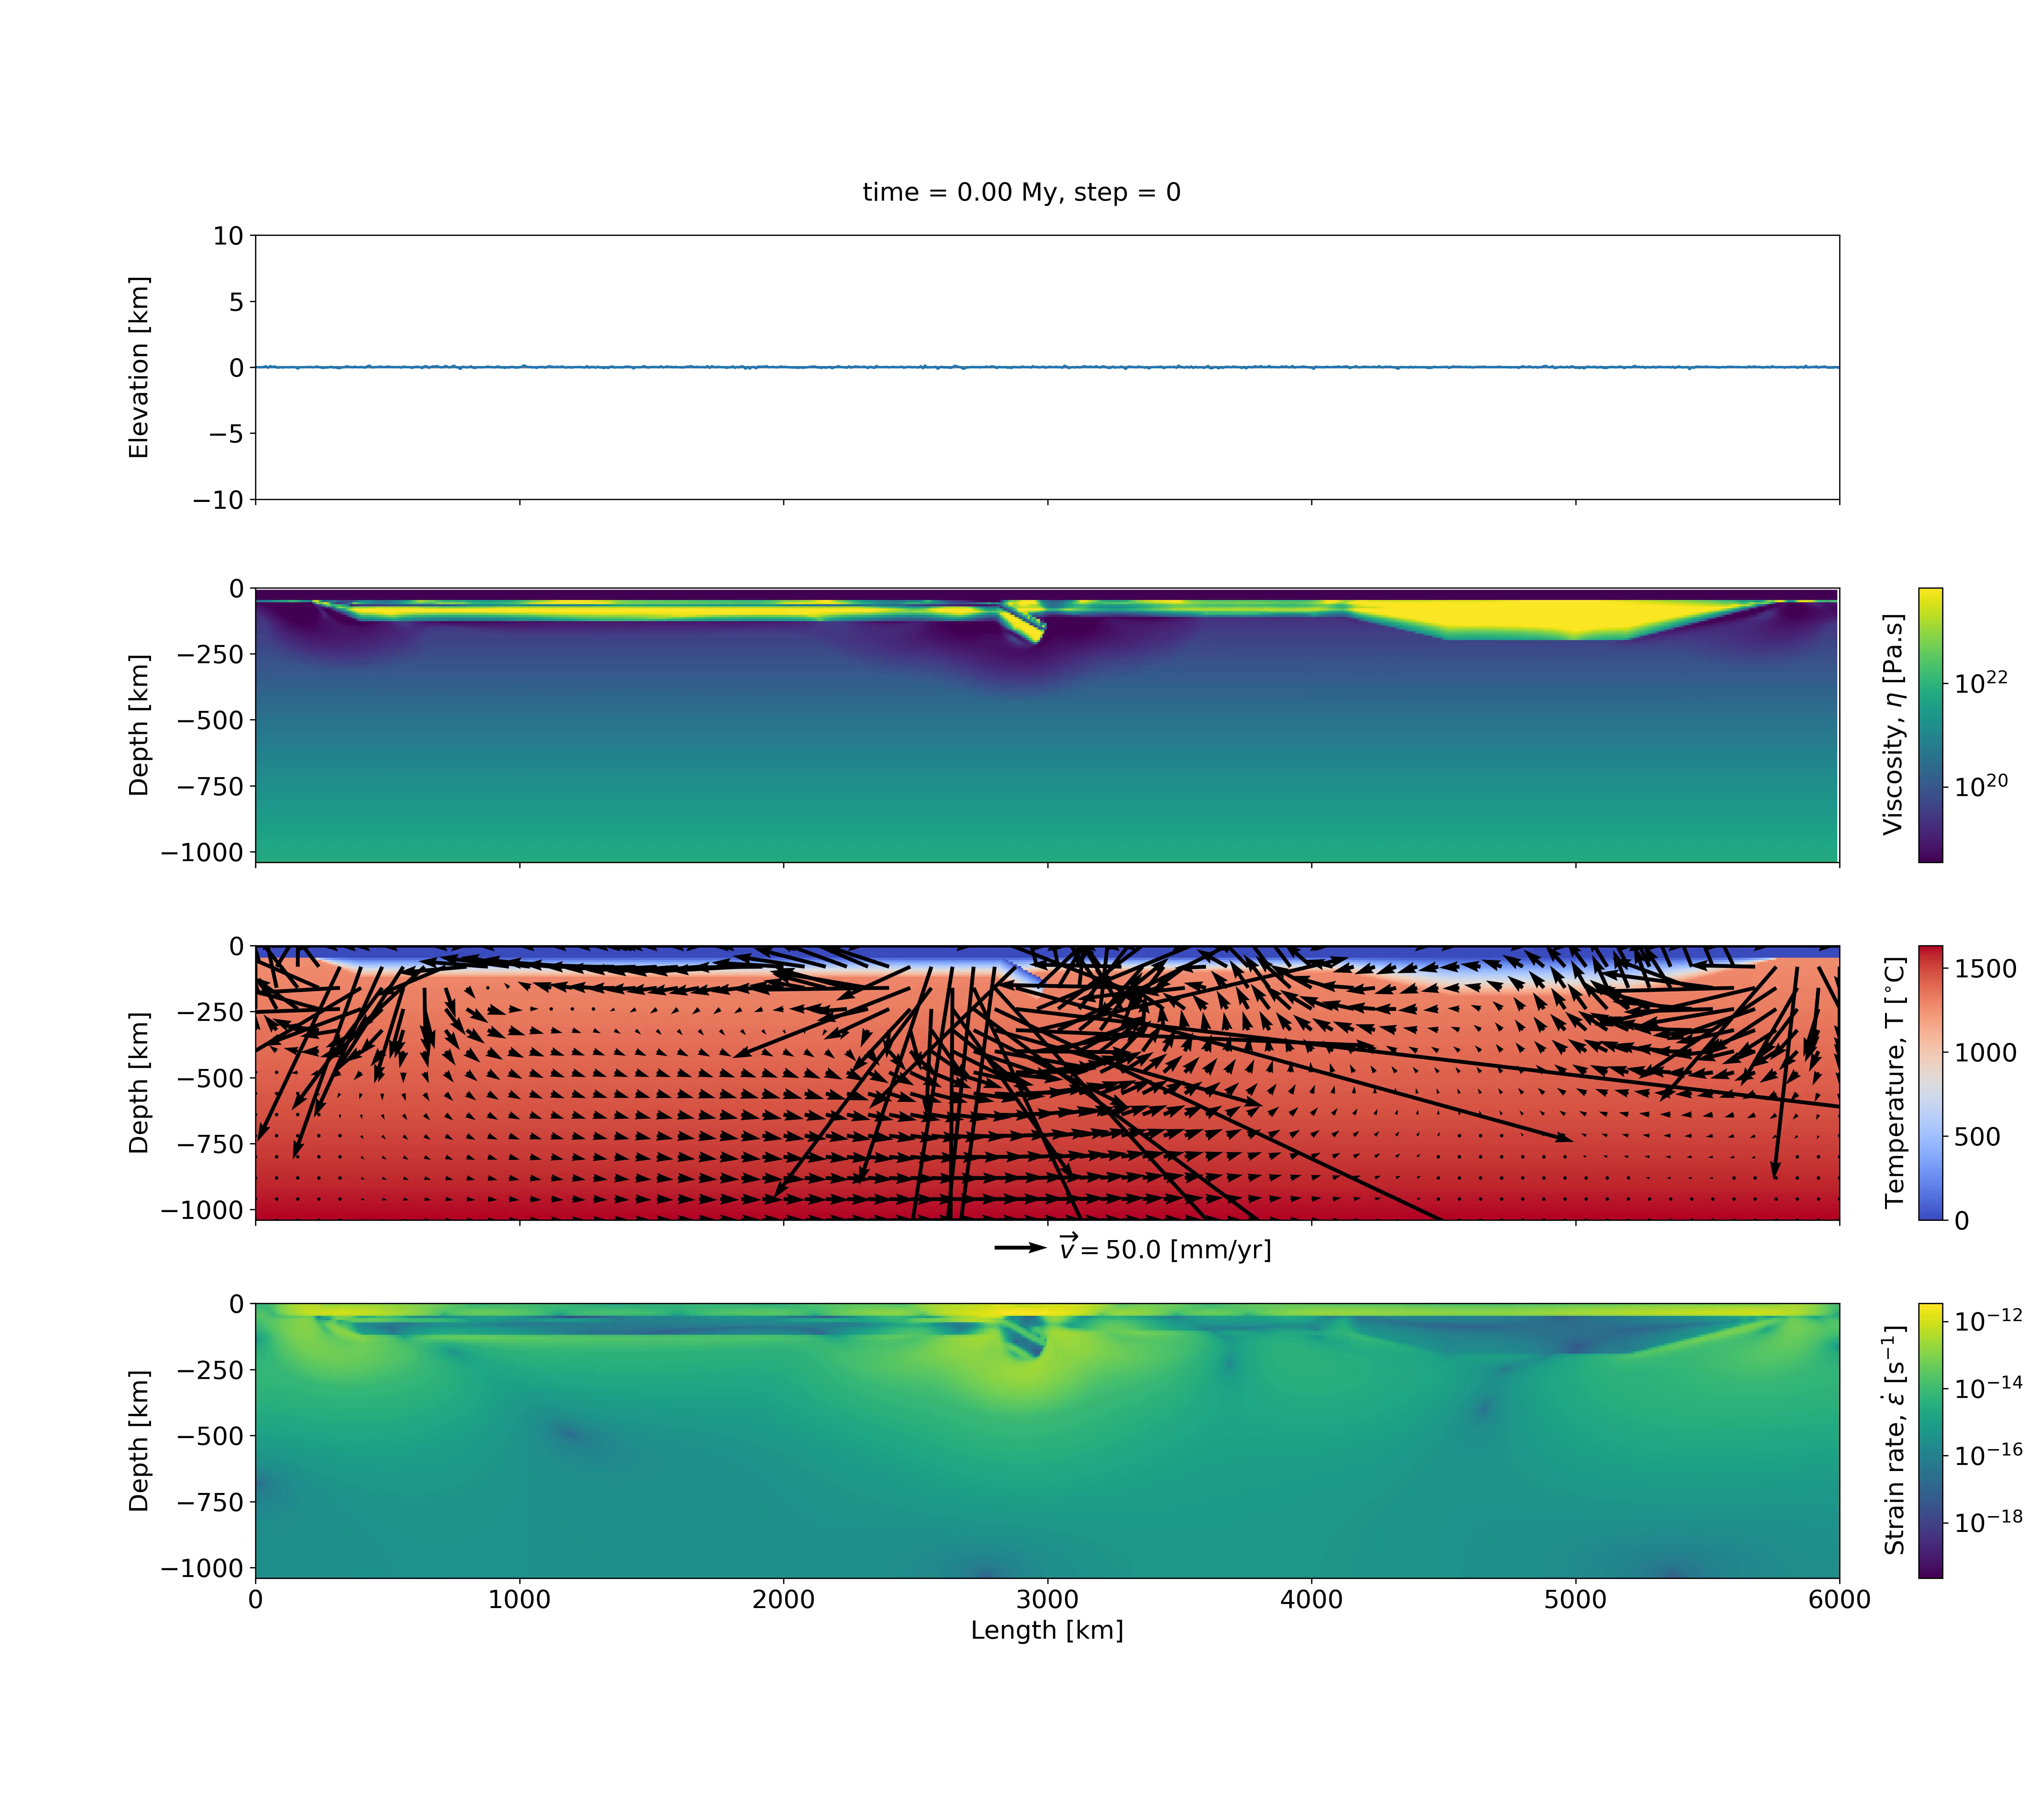
\includegraphics[trim={5cm 14cm 2cm 12cm}, clip, width=1.0 \textwidth]{fig/strak_32-00.png}
    \caption{Configuração inicial do Modelo de Referência. De cima para baixo, as figuras representam a topografia, campo de viscosidade, campo de velocidade sobreposto ao campo de temperatura, e campo de taxa de deformação.}
    \label{fig:strak_32-00}
\end{figure}

\begin{figure}
    \centering
    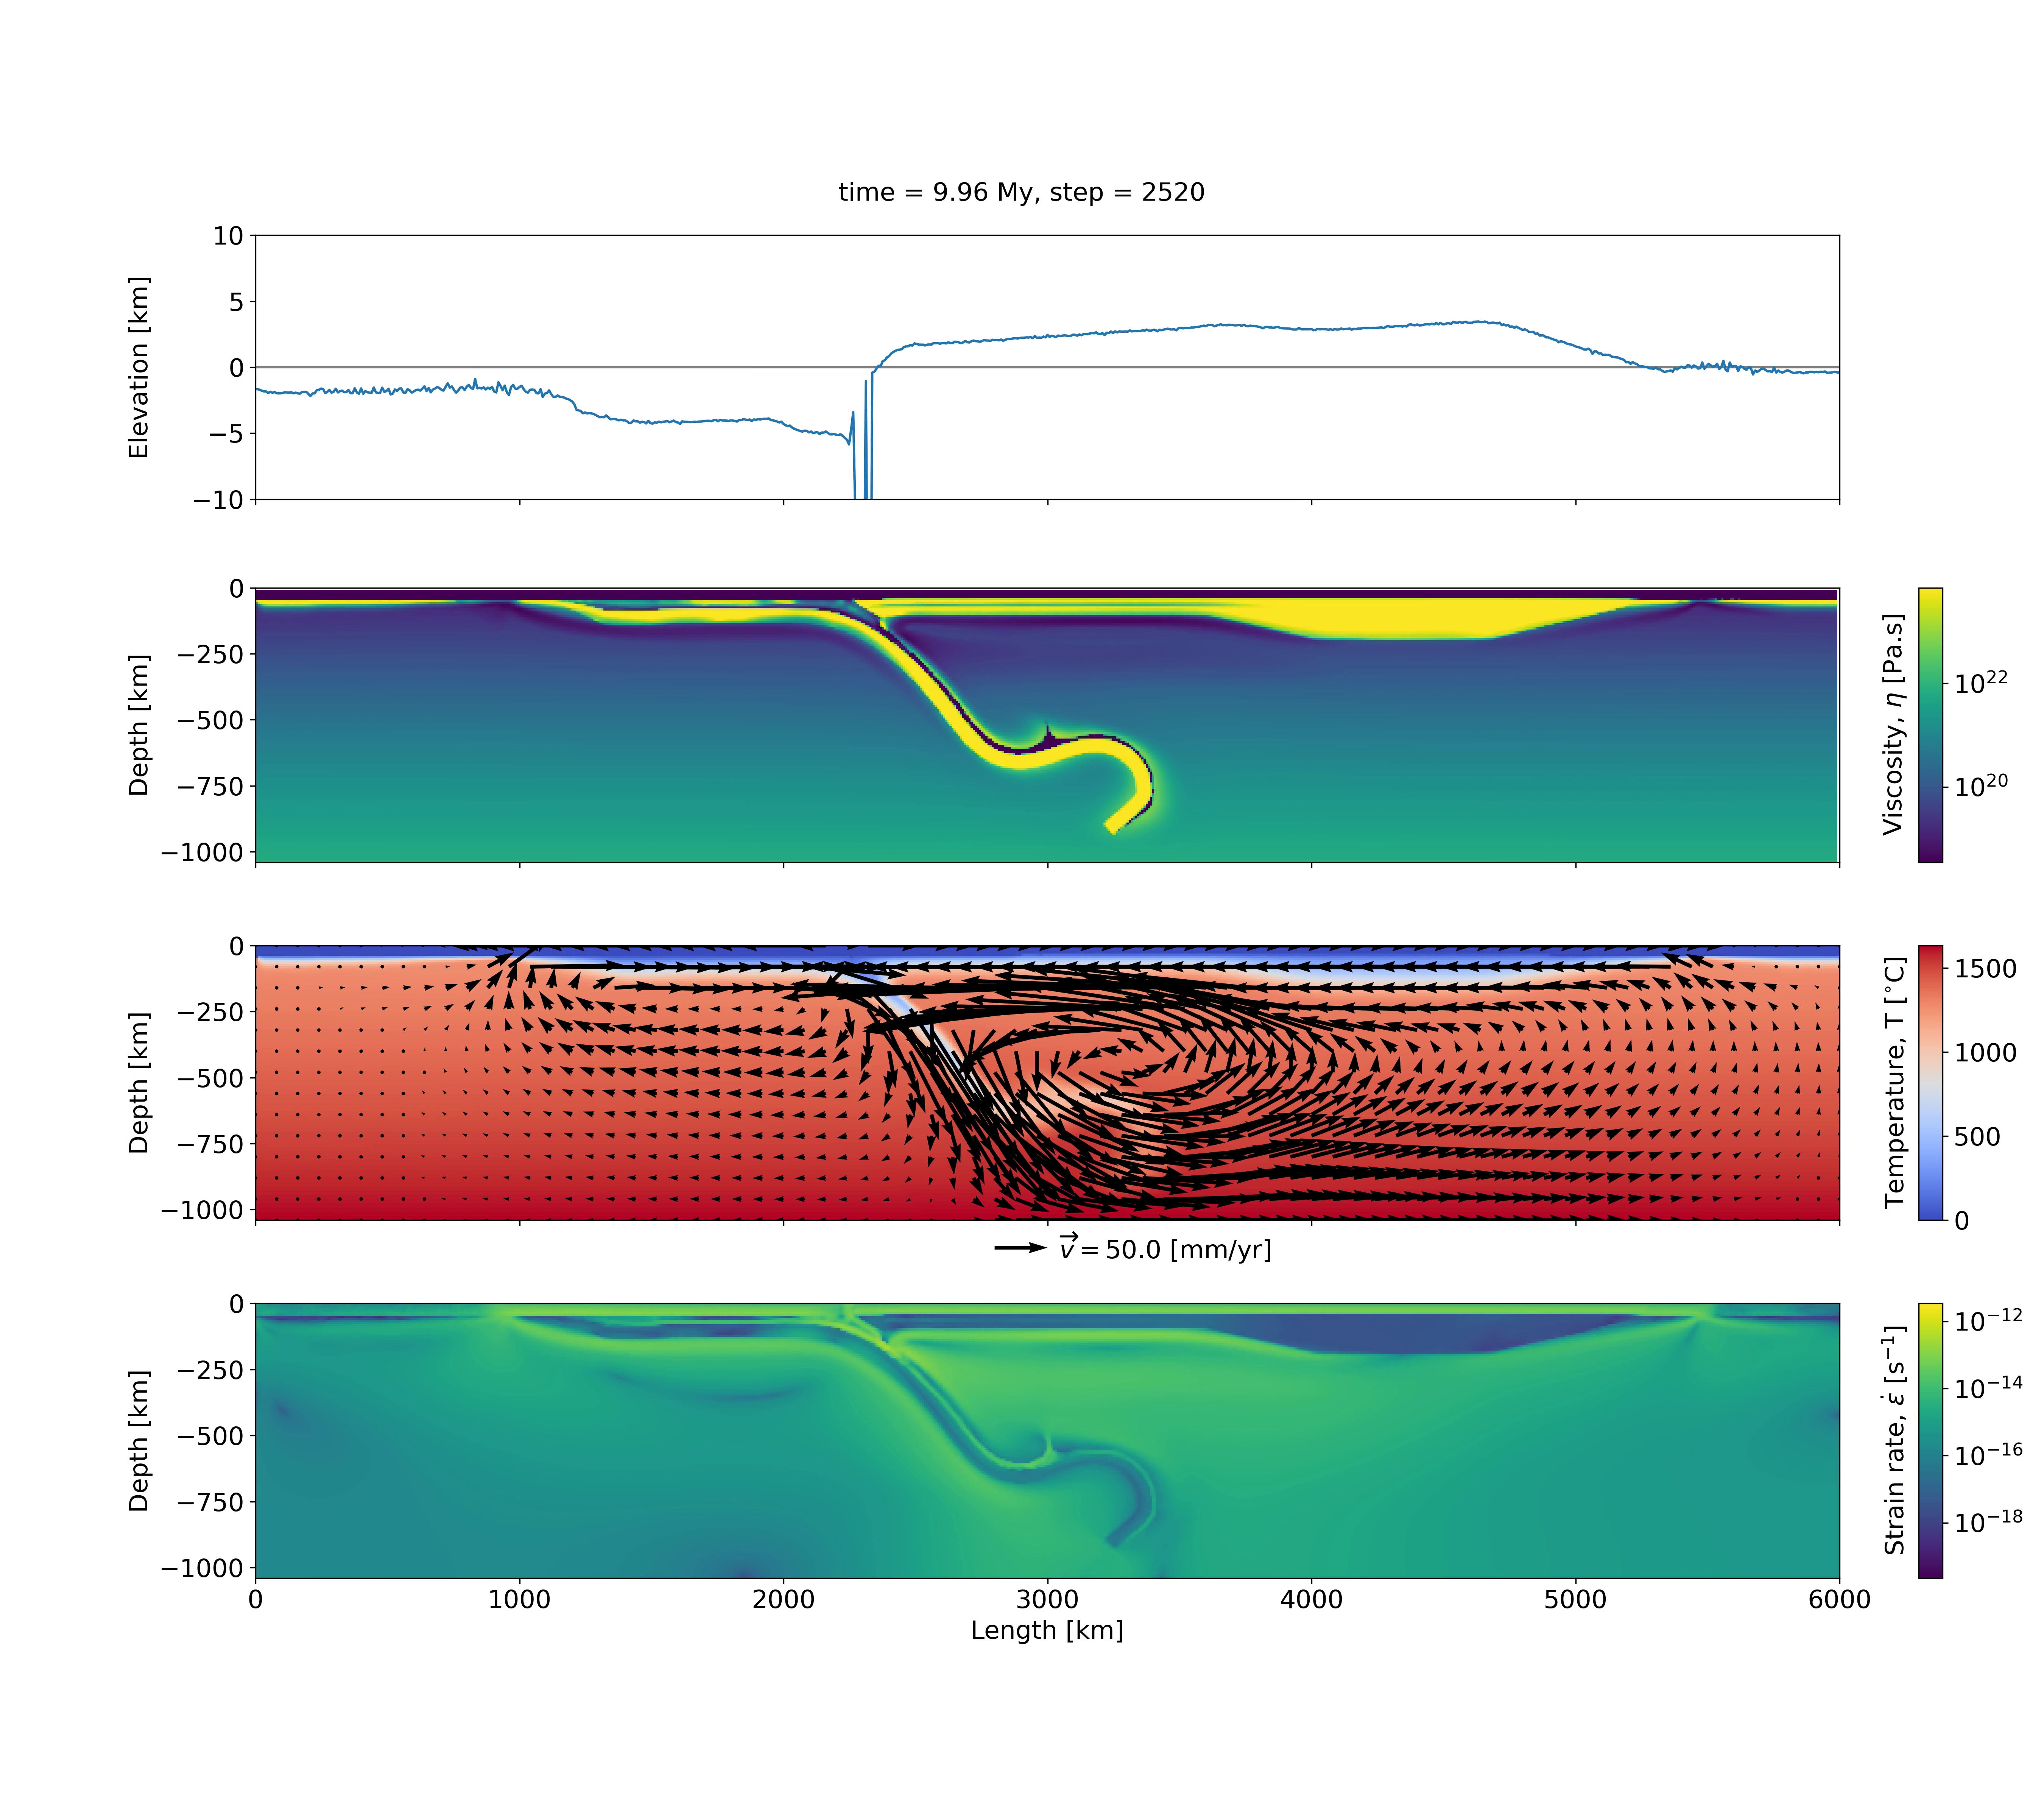
\includegraphics[trim={5cm 14cm 2cm 12cm}, clip, width=1.0 \textwidth]{fig/strak_32-11.png}
    \caption{Configuração do Modelo de Referência após $9.96$ Ma. De cima para baixo, as figuras representam a topografia, campo de viscosidade, campo de velocidade sobreposto ao campo de temperatura, e campo de taxa de deformação.}
    \label{fig:strak_32-11}
\end{figure}

Outras simulações utilizaram abordagens diferentes para simular subdução e não serão mostradas aqui. Um conjunto dessas simulações, por exemplo, utilizou uma litosfera continental fragilizada de $50$ km de largura no contato com a litosfera oceânica em subdução, criando uma zona lubrificante. A utilização de uma zona lubrificante permitiu subdução consistentemente, no entanto a abordagem de crosta oceânica fragilizada é mais simples e coerente com a geologia.

Para o MR, a subdução ocorre sem haver acoplamento da litosfera oceânica com a litosfera continental, figuras \ref{fig:strak_32-00} e \ref{fig:strak_32-11}. Para que ocorra subdução, no entanto, há necessidade de uma crosta oceânica fragilizada e menos viscosa conforme outras simulações mostraram. \citet{strak2021thermo} utilizaram três camadas para a litosfera oceânica, duas para a crosta e uma para o manto litosférico. A abordagem no MR é inicialmente mais simples, ele usa apenas uma camada para a crosta e uma para o manto litosférico e também uma crosta oceânica relativamente menos viscosa. Após $9.96$ Ma, a simulação apresenta uma placa descendente coesa em profundidade e com uma trajetória que indica maiores velocidades no meio da placa em comparação com a sua extremidade direita, causando dobramento da litosfera em subdução.

As figuras \ref{fig:strak_32-00} e \ref{fig:strak_32-11} mostram que também ocorre expressivo avanço da litosfera continental, da direita para a esquerda, ao longo de $\sim500$ km. Nota-se ainda que a porção cratônica se mantém estável durante a simulação e os esforços diminuem na porção de arco continental. Nas laterais do modelo, onde inicialmente não havia litosfera, uma proto-litosfera se desenvolve.

Como o modelo não está em equilíbrio isostático desde o início da simulação, ocorre uma subsidência da porção oceânica e um soerguimento da porção continental, com a posição da trincheira bem definida, porém sem orogenia da porção esquerda da litosfera continental, como mostra o gráfico de elevação na figura \ref{fig:strak_32-11}.

O padrão de convecção observado no gráfico de campo de velocidade (figura \ref{fig:strak_32-11}) indica uma grande célula de convecção que rotaciona no sentido horário sob a região da placa oceânica. Sob a litosfera continental, o manto apresenta convecção vigorosa na região de arco continental, no sentido anti-horário, e a célula de convecção alcança a extremidade direita da placa continental.

O MR utiliza uma crosta oceânica bastante densa e espessa, e simulações posteriores com crosta oceânica mais finas ($8$, $10$ e $15$ km) não apresentaram subdução. A suspeita inicial foi de que a resolução do modelo não era suficiente para que as camadas tivessem o comportamento reológico esperado, mas simulações posteriores não validaram essa hipótese. Uma abordagem usando um modelo de resfriamento de placa \citep{turcotte2002geodynamics} também foi testada para quantificar o efeito do \textit{ridge-push}, mas outros testes ainda precisam ser realizados.

% [WIP] Modelos cuja crosta oceânica era muito mais fina não apresentaram subdução. Modelos cuja crosta oceânica apresentava densidade menor não apresentaram subdução. Modelos usando modelo de resfriamento de placa teoricamente teriam \textit{ridge-push} ao longo de uma região maior, mas não ajudaram muito (por enquanto).

% [WIP] strain seed na crosta oceânica subduzida (COS) e na crosta oceânica não-subduzida (CONS). Fator composicional da COS e da CONS é 0.01.

Um segundo modelo (SM) é mostrado nas figuras \ref{fig:stra_52-00} e \ref{fig:stra_52-11} após $9.81$ Ma. O intuito deste modelo teste é entender como o fator composicional e a fragilização afetam o processo de subdução lateralmente. Nesta simulação, no entanto, a largura do modelo, e consequentemente da litosfera oceânica e litosfera continental, foi diminuída para um domínio de $5000$ km. Além disso, o número de elementos finitos passou a ser $(nx\times ny)=(800\times 160)$. Essas diferenças devem ter impacto negligenciável no resultado final deste segundo modelo. O que deve impactar o modelo são as mudanças feitas à crosta oceânica, que agora foi dividida em dois domínios: um horizontal e outro em subdução, tal como mostra a figura \ref{fig:geometria-inicial}. Essa divisão foi feita para utilizar dois regimes reológicos diferentes na mesma crosta oceânica. Enquanto os parâmetros para a porção em subdução são os mesmos do MR, a porção horizontal apresenta um fator composicional $C=1.00$ e não é fragilizada. Um vídeo completo da simulação pode ser visualizado em \url{https://youtube.com/shorts/qI9AQq6iqwY?feature=share}.

\begin{figure}
    \centering
    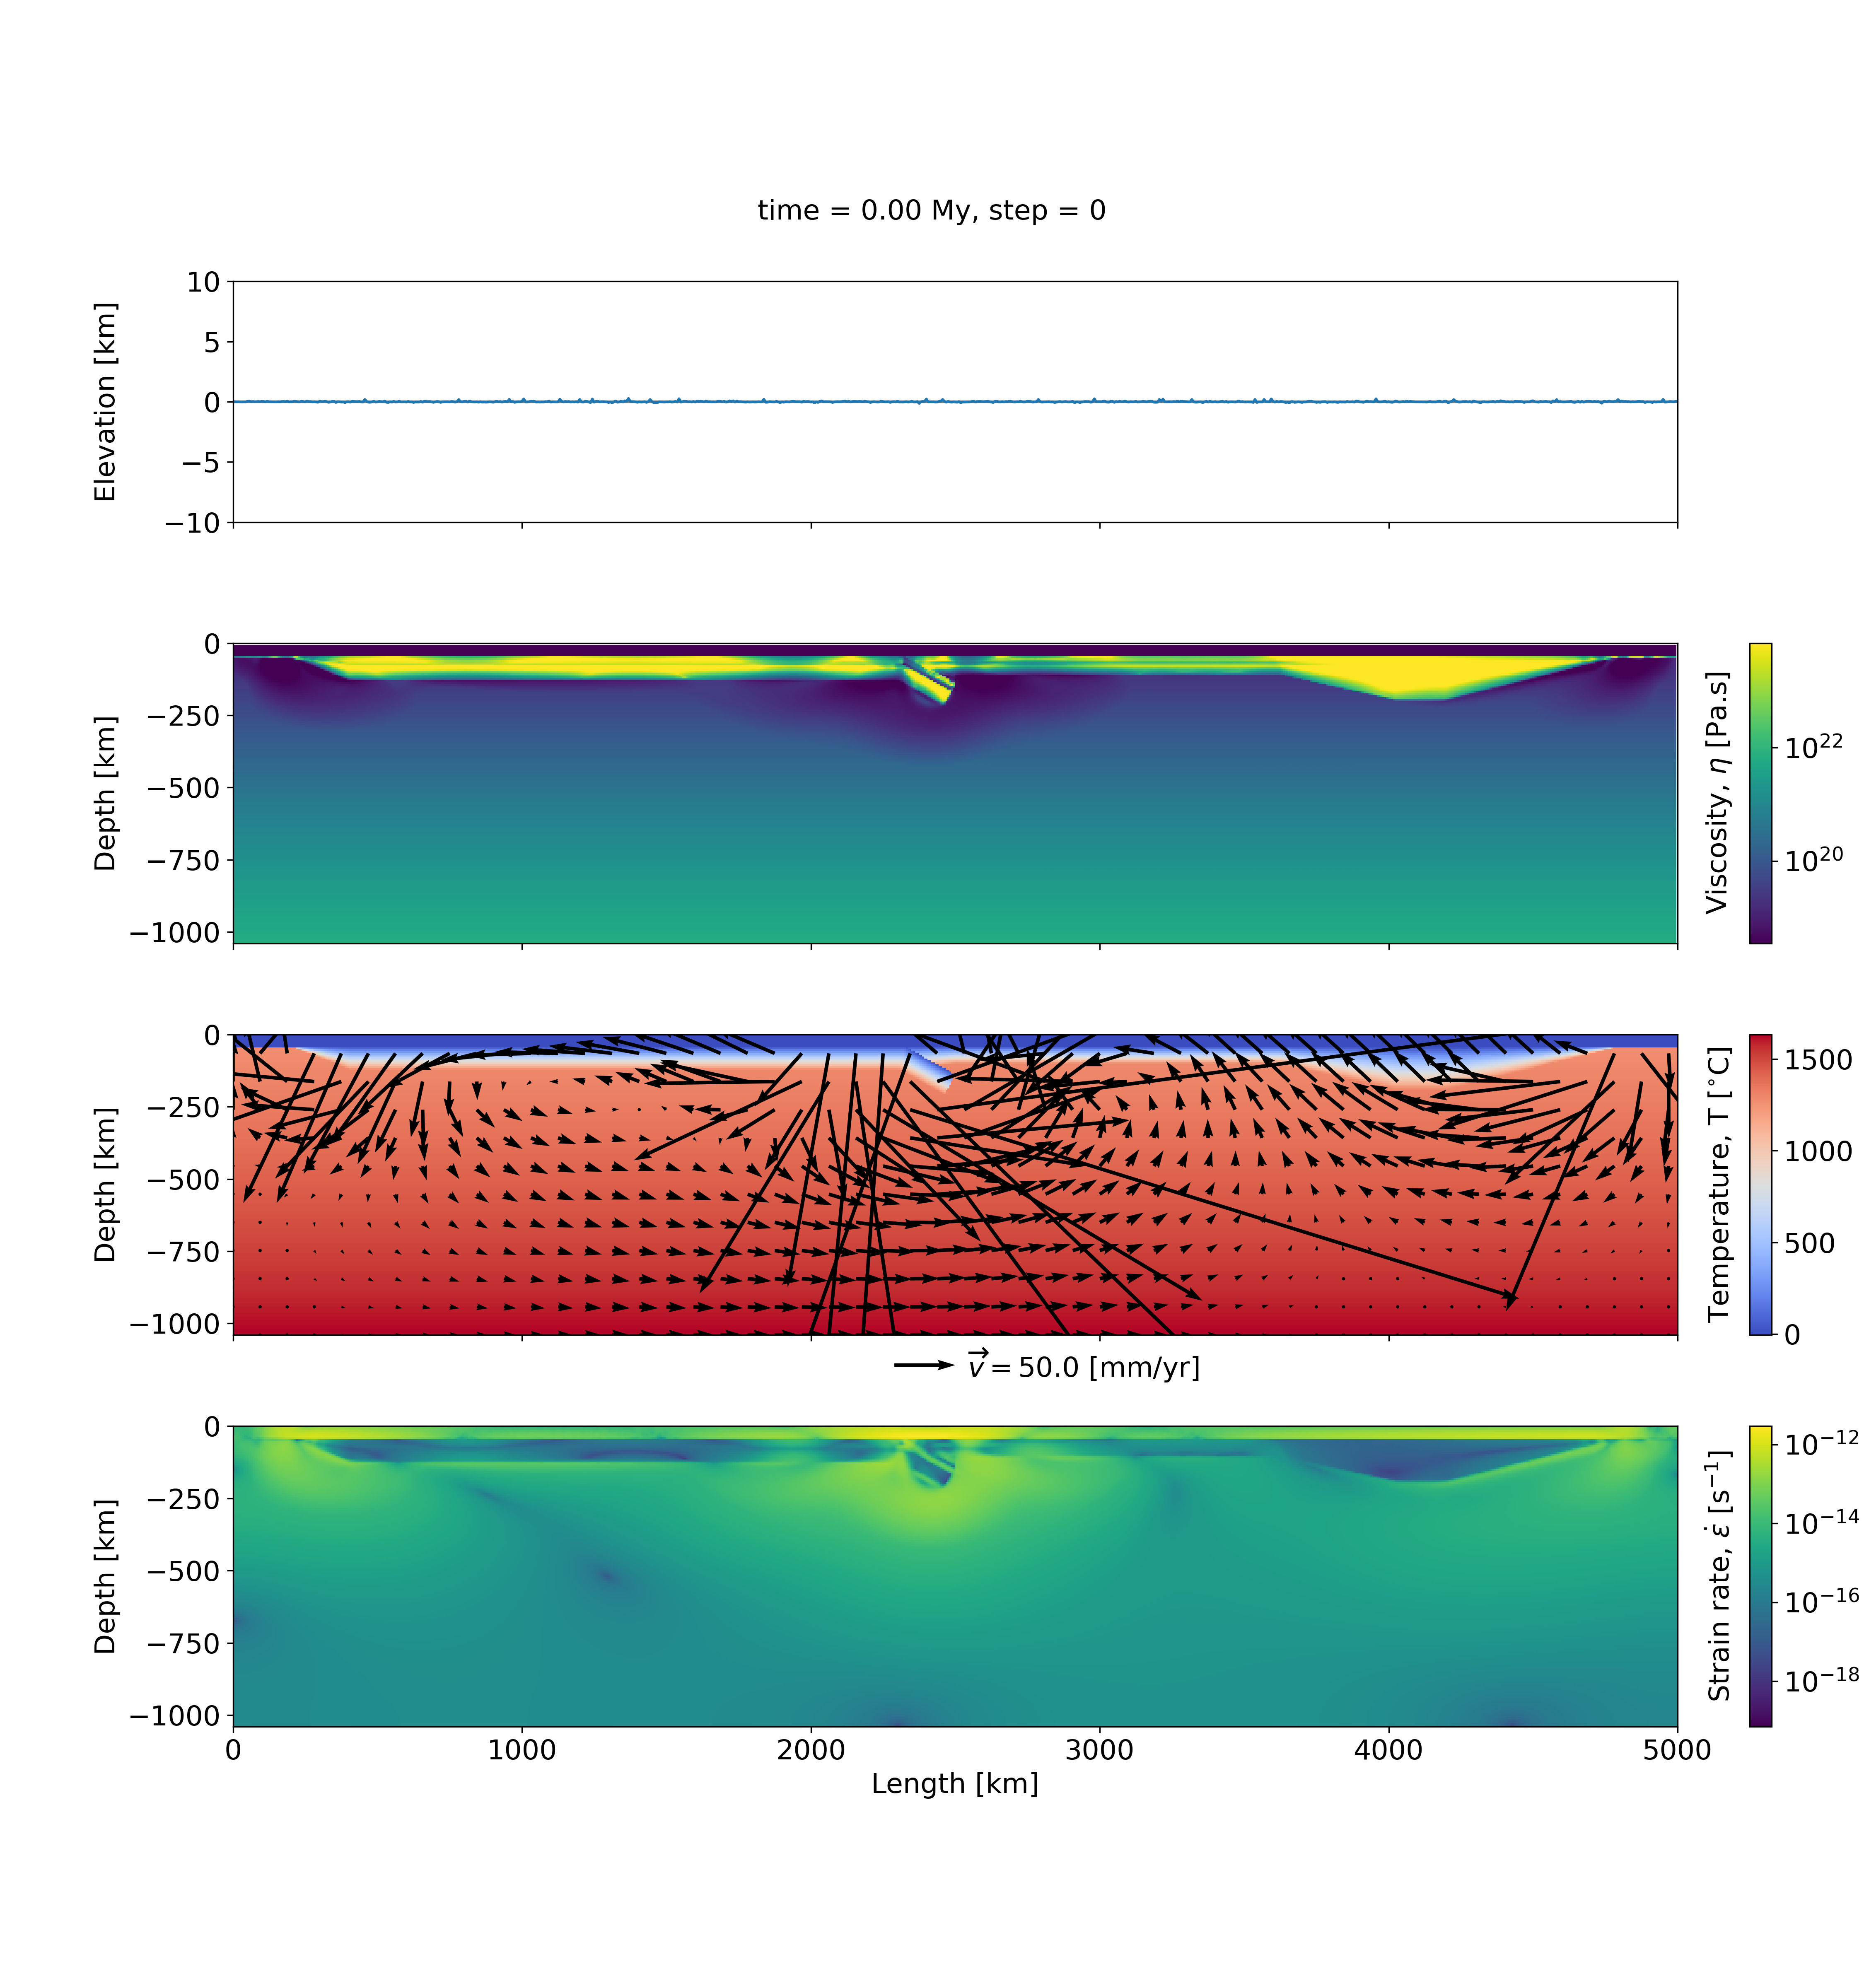
\includegraphics[trim={1.5cm 3.5cm 0.0cm 4cm}, clip, width=1.0 \textwidth]{fig/strak_52-00.png}
    \caption{Configuração inicial do Modelo 52. De cima para baixo, as figuras representam a topografia, campo de viscosidade, campo de velocidade sobreposto ao campo de temperatura, e campo de taxa de deformação.}
    \label{fig:stra_52-00}
\end{figure}

\begin{figure}
    \centering
    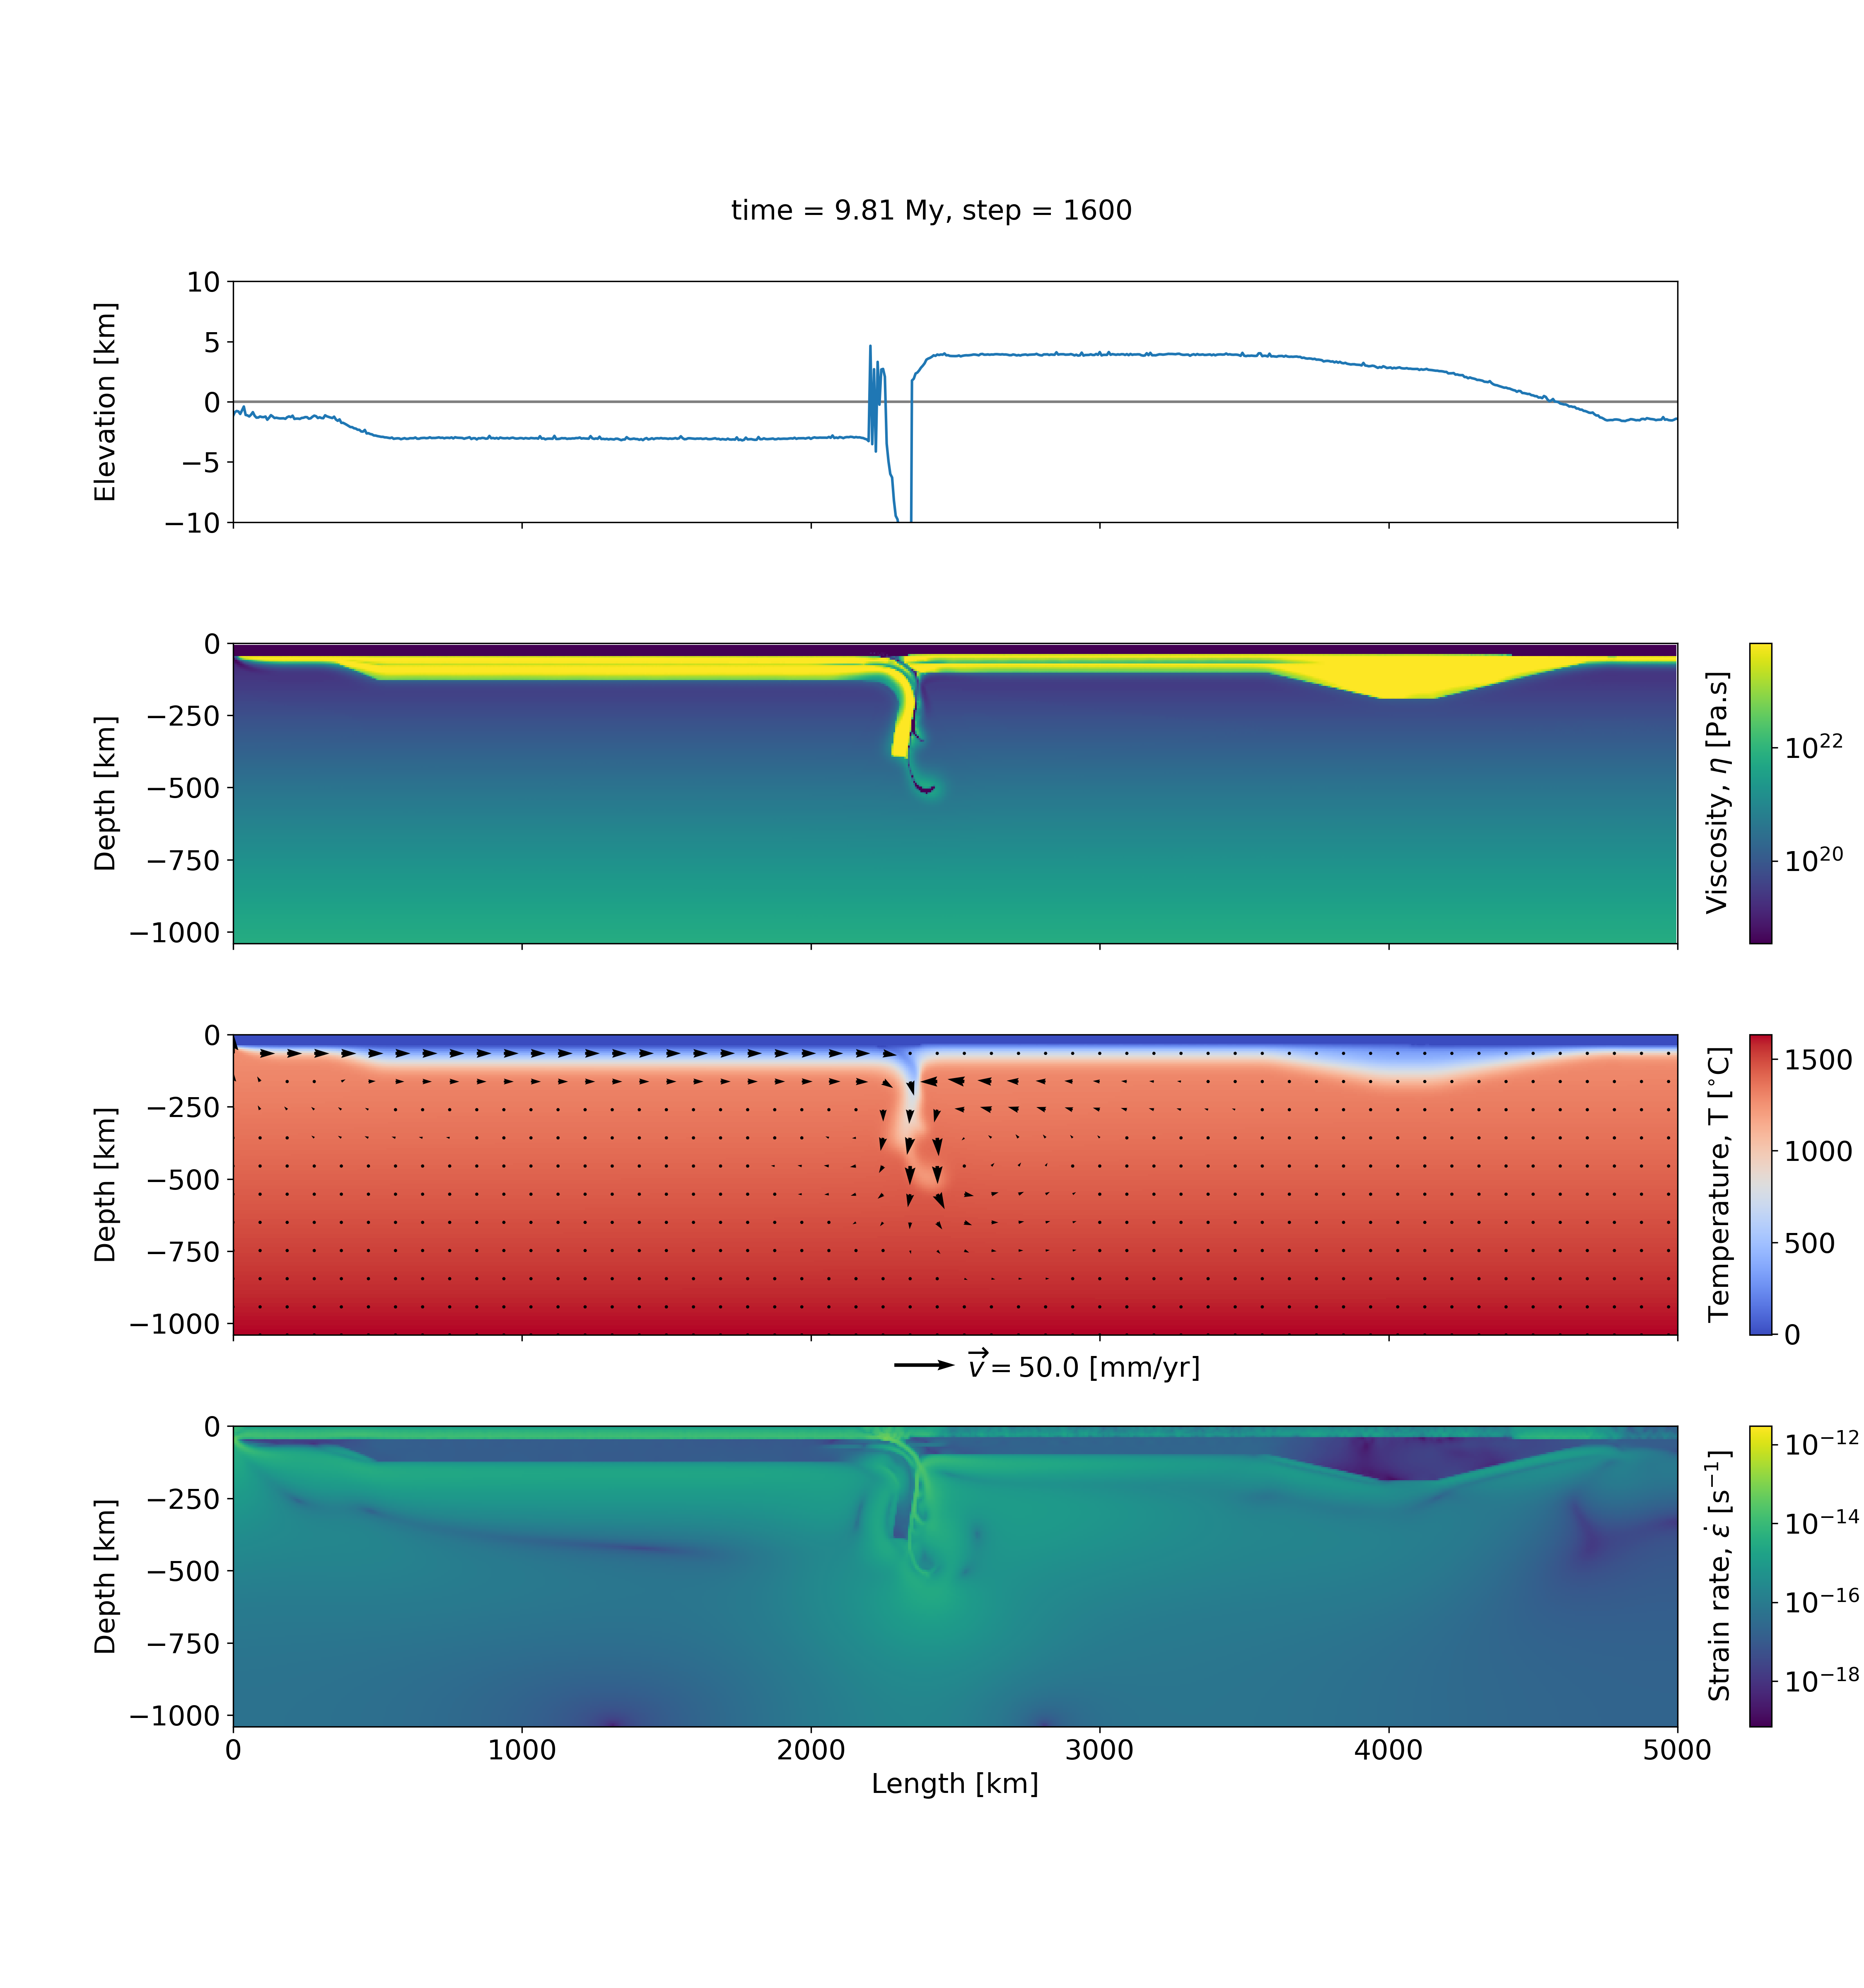
\includegraphics[trim={1.5cm 3.5cm 0.0cm 4cm}, clip, width=1.0 \textwidth]{fig/strak_52-11.png}
    \caption{Configuração do Modelo 52 após $9.81$ Ma. De cima para baixo, as figuras representam a topografia, campo de viscosidade, campo de velocidade sobreposto ao campo de temperatura, e campo de taxa de deformação.}
    \label{fig:stra_52-11}
\end{figure}

A subdução do SM não é total e, de fato, é interrompida. Esse resultado mostra que a crosta de contato é capaz de permitir que a subdução ocorra, mas a crosta oceânica não fragilizada impede que a subdução continue. Ainda, a simulação como um todo apresenta células de convecção menos vigorosas do que o MR.

Nesta segunda simulação, no entanto, há maior elevação da topografia na porção esquerda da litosfera continental, 

% [WIP] strain seed apenas na COS. Fator composicional da COS é 0.01 e da CONS é 1.0.

Em um terceiro modelo (TM), todos os parâmetros são os mesmos do SM, exceto que agora a crosta oceânica inteira apresenta fator composicional $C=1.00$ e fragilização. O resultado da simulação após $9.91$ Ma é mostrado na figura \ref{fig:stra_53-11}. Um vídeo completo da simulação pode ser visualizado em \url{https://youtube.com/shorts/pG0MjPCSBXY?feature=share}.

% \begin{figure}
%     \centering
%     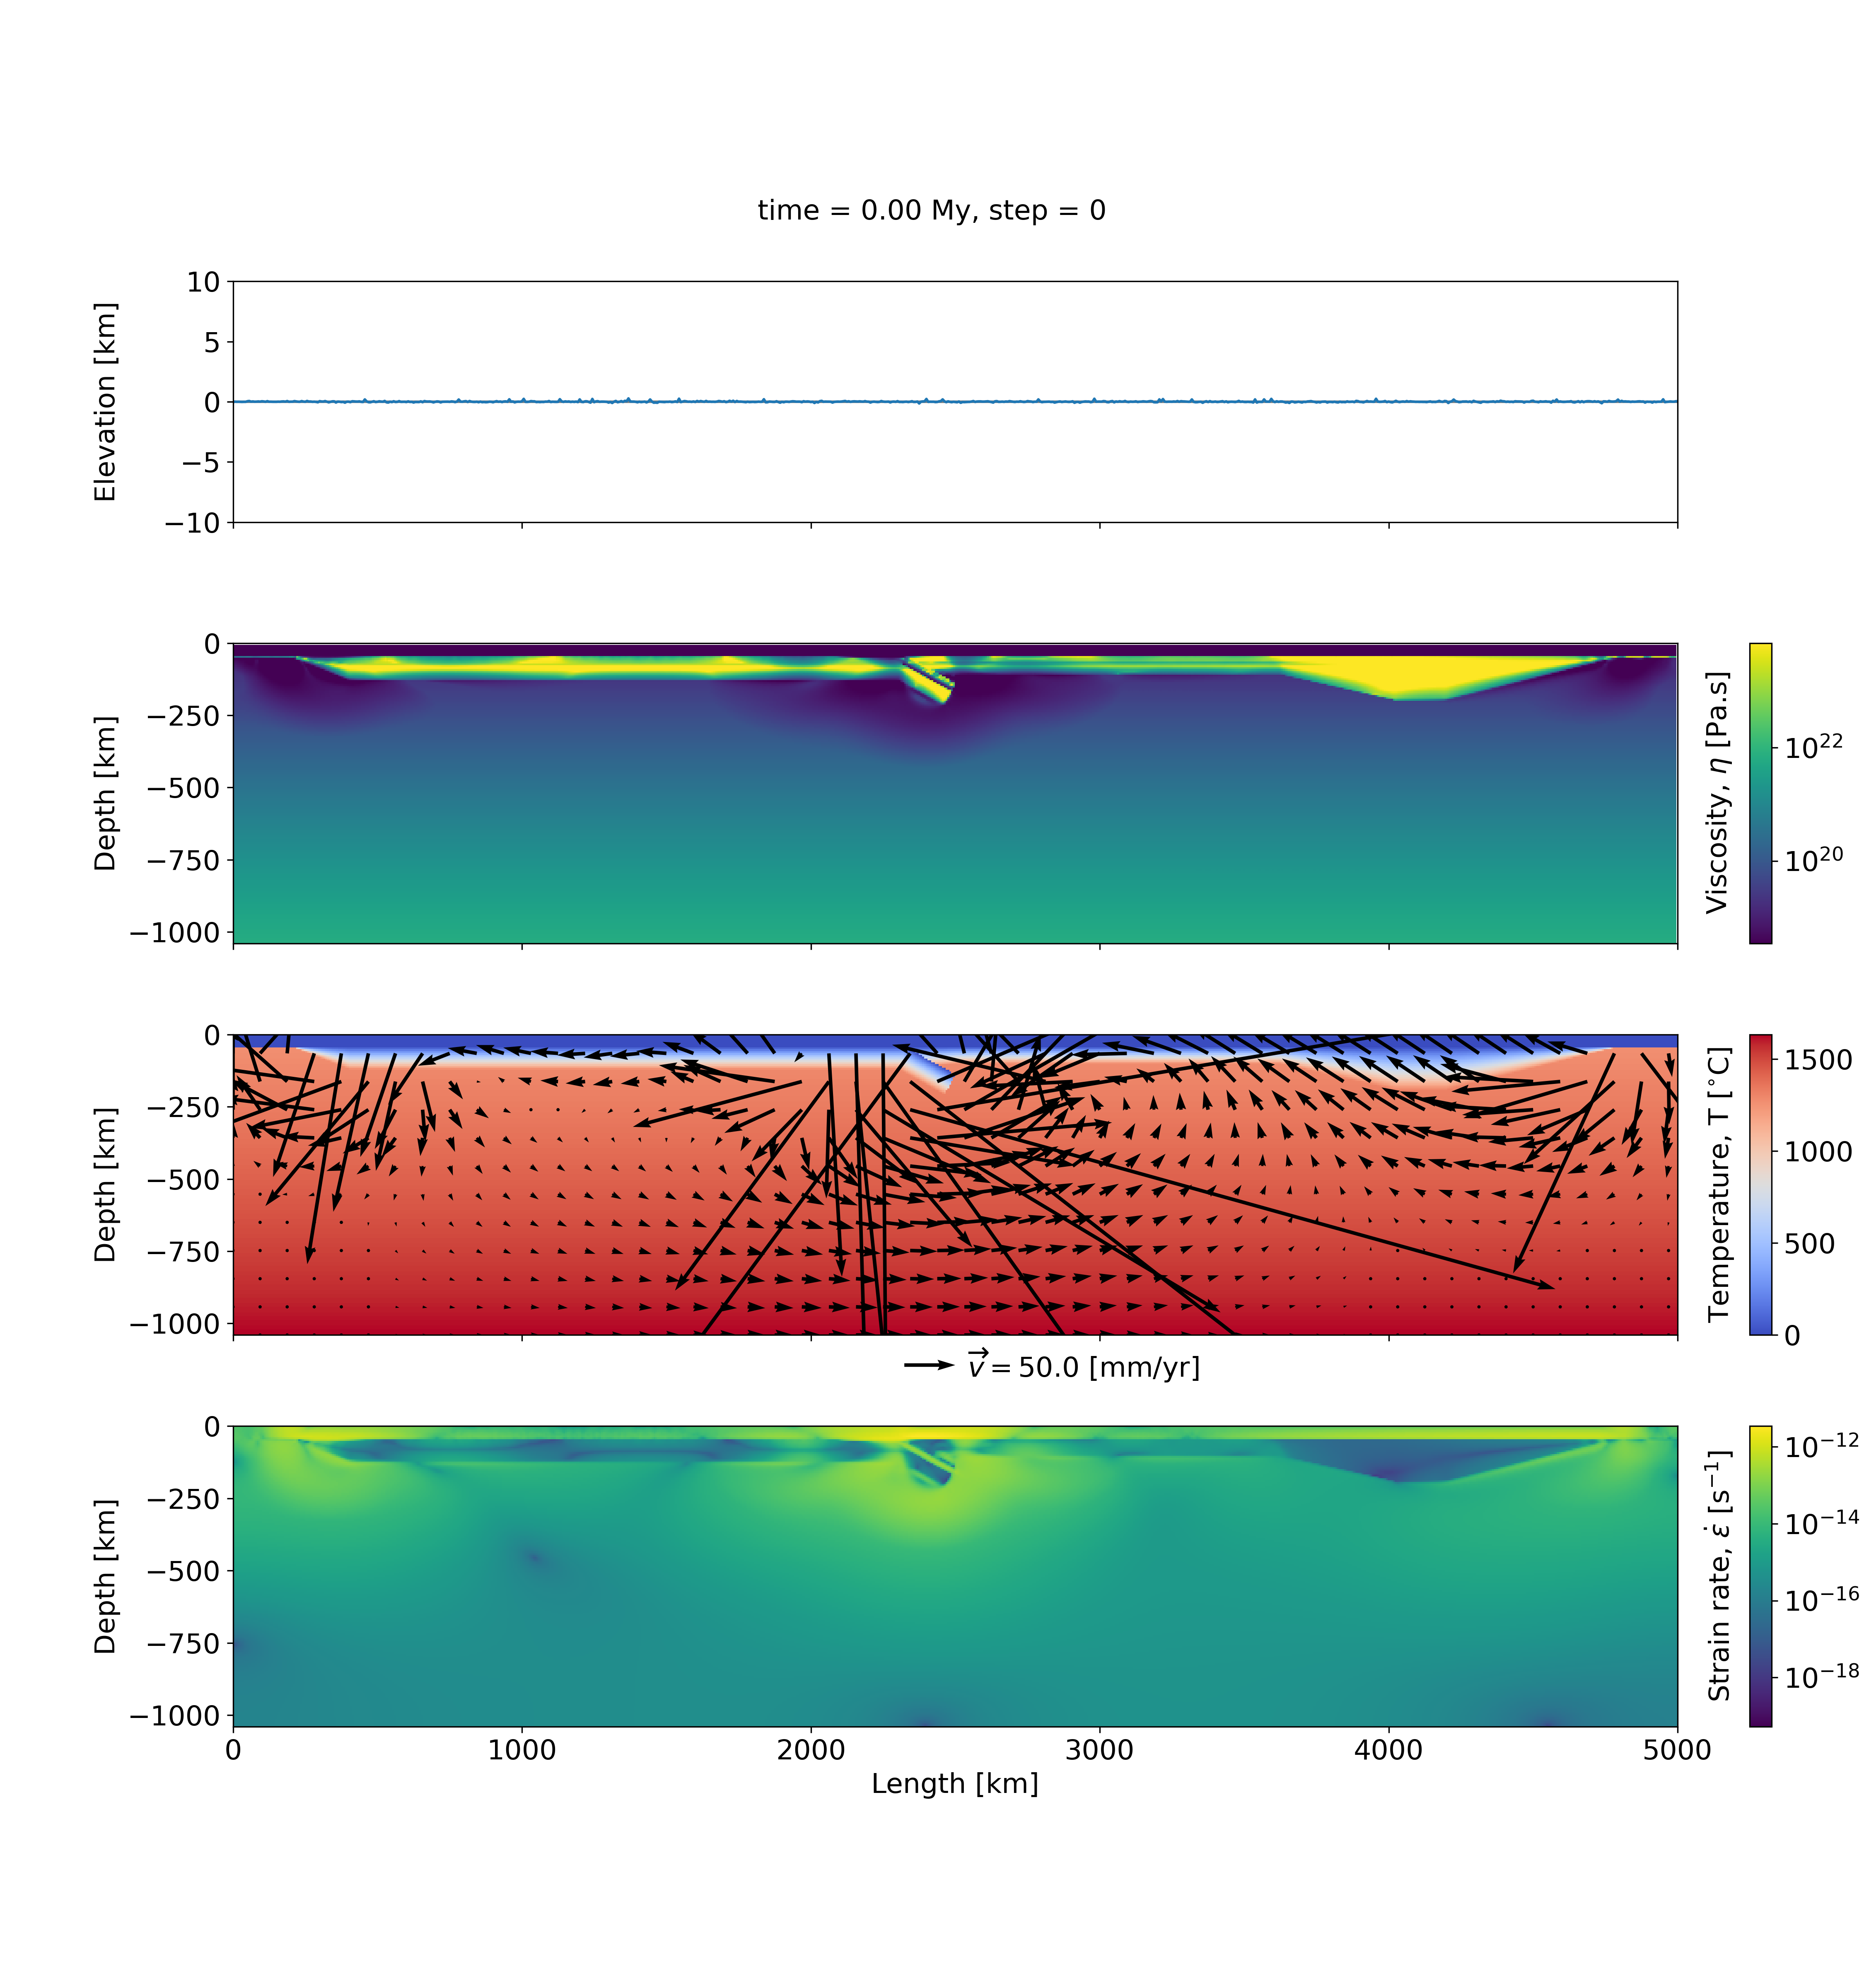
\includegraphics[trim={1.5cm 3.5cm 0.0cm 4cm}, clip, width=1.0 \textwidth]{fig/strak_53-00.png}
%     \caption{Configuração inicial do Modelo 53. De cima para baixo, as figuras representam a topografia, campo de viscosidade, campo de velocidade sobreposto ao campo de temperatura, e campo de taxa de deformação.}
%     \label{fig:stra_53-00}
% \end{figure}

\begin{figure}
    \centering
    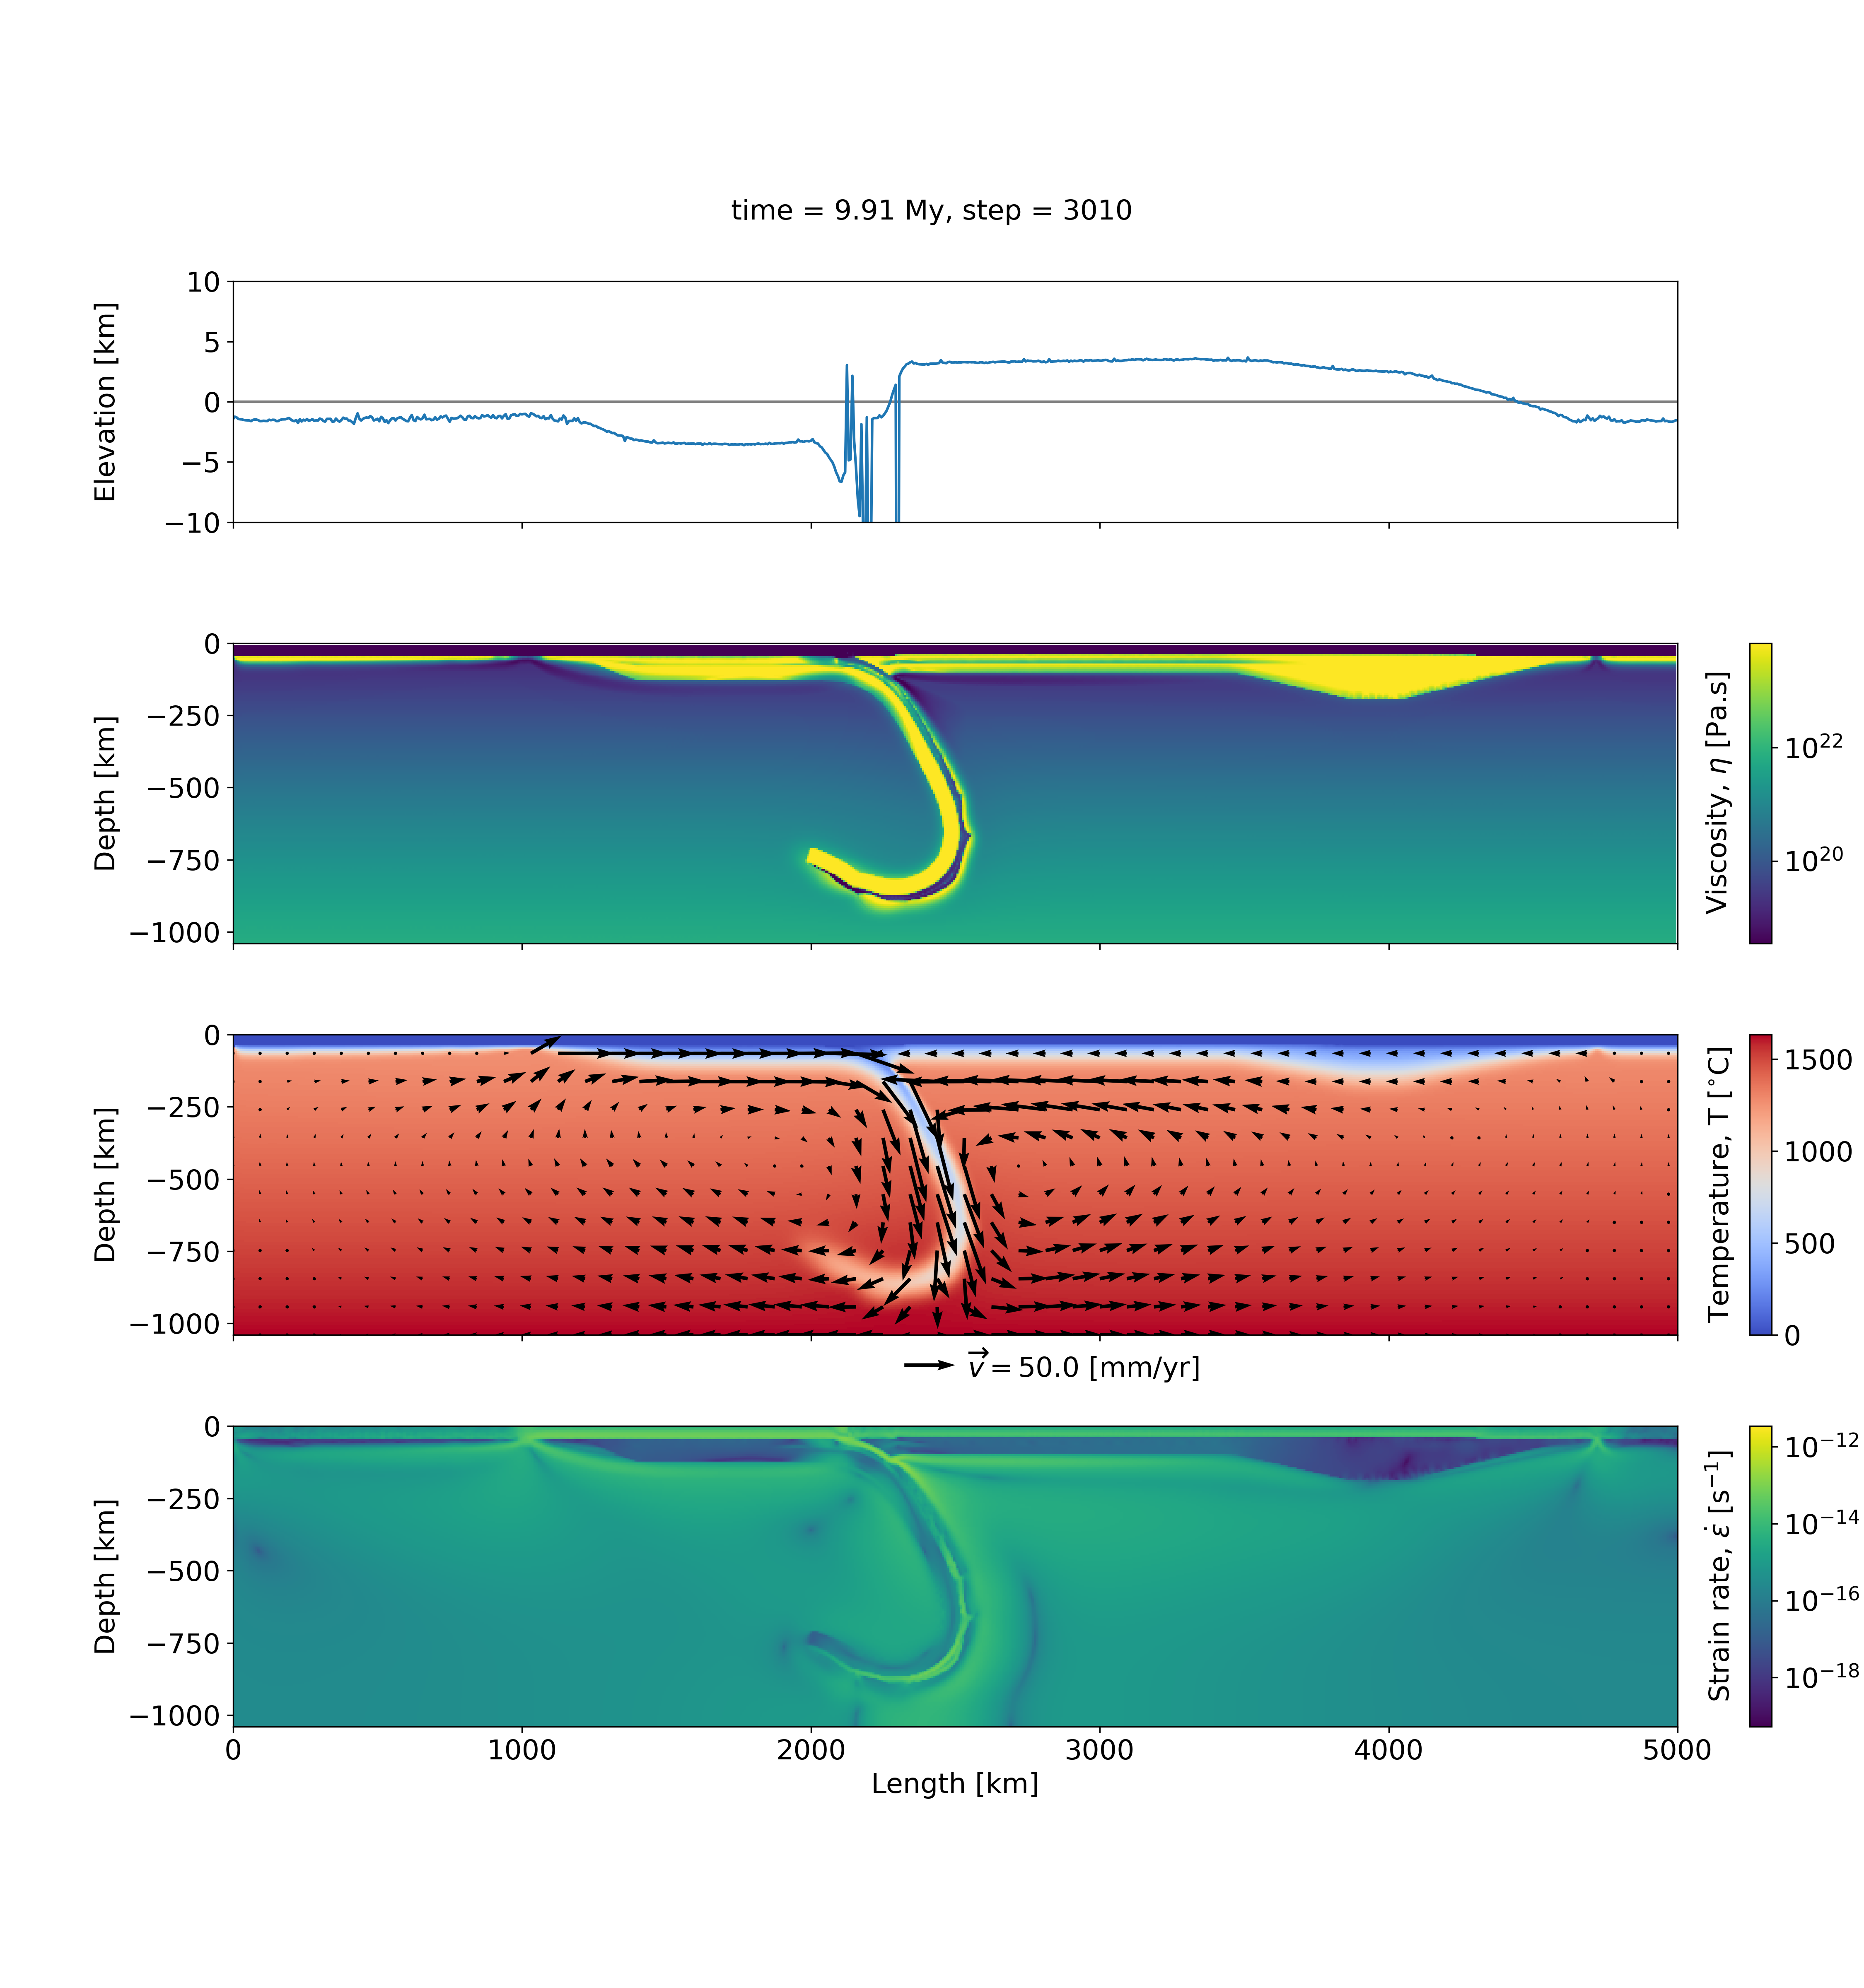
\includegraphics[trim={1.5cm 3.5cm 0.0cm 4cm}, clip, width=1.0 \textwidth]{fig/strak_53-11.png}
    \caption{Configuração do Modelo 53 após $9.91$ Ma. De cima para baixo, as figuras representam a topografia, campo de viscosidade, campo de velocidade sobreposto ao campo de temperatura, e campo de taxa de deformação.}
    \label{fig:stra_53-11}
\end{figure}

% [WIP] strain seed na COS e na CONS. Fator composicional da COS é 0.01 e da CONS é 1.0.

O conjunto de simulações SM e TM sugerem que a fragilização é mais importante do que o fator composicional na ocorrência de subdução. O conjunto total de simulações (MR, SM e TM) também mostram que o desenvolvimento da topografia na litosfera continental é mais expressivo se há maior acoplamento entre as placas. 
% Ou seja, orogenia na porção esquerda da crosta continental está associada ao acoplamento durante a subdução, de tal forma que se a subdução ocorre sem dificuldades, menor será a evolução topográfica na litosfera sobrejacente.









